\chapter{Introduction}
\label{chap2}

Project eXpOS or experimental Operating System is a educational platform to develop an operating system. Several instructional operating systems like Nachos, Pintos, GeekOS etc. have been developed by various universities for this purpose.
Nachos has been one of the most popular instructional operating systems available and is being used in many institutes across the world. XOS, the previous version of eXpOS, was such a tool that helps undergraduate computer science students acquire an elementary understanding of the practical aspects of an operating system.
\\
XOS had features like multiprogramming, process management, a primitive filesystem and virtual memory. In order to incorporate simplicity, OS features like inter-process communication, device management, file caching, file permissions etc. had been excluded from XOS. In the present version, eXpOS, some of these features such as inter process communication, asynchronous disk access, heap memory, etc had been included to make the student more proficient in Operating System concepts. The basic Machine model consists of memory, disk and the CPU. eXpOS includes specification for a set of system calls, the scheduler, the exception handler, device drivers etc.  Further hardware support required includes the timer, disk controller, Input-output system etc.
\\
The primary components of the project include a simulated machine hardware (XSM), file system (eXpFS) and the operating system (eXpOS). No code base for the operating system is provided and the operating system is completely implemented by the student. Apart from the primary components, various tools are provided as part of the development environment. They include languages like Experimental Programming Language (ExpL) and System Programmer's Language (SPL) and their cross compilers to XSM instruction set, XSM debugger, and a UNIX-XFS interface to transfer files between a UNIX machine and the XFS disk (the eXpFS disk is itself a UNIX file). Generic hardware model is described below.

\begin{figure}[ht]
\centering
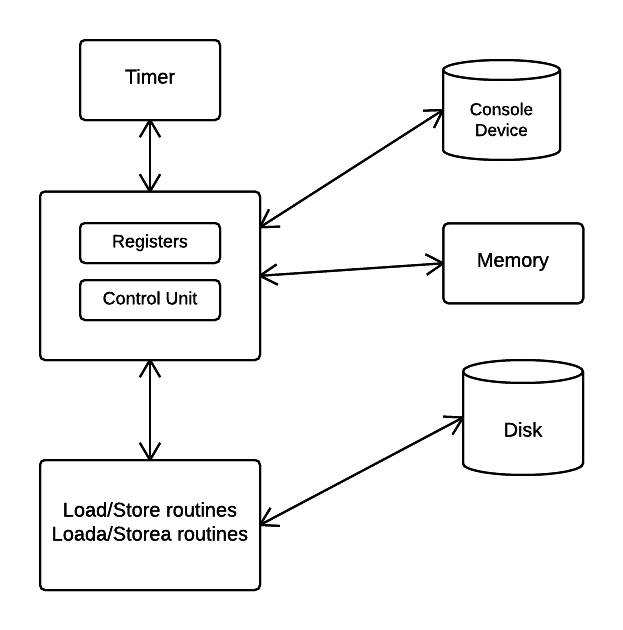
\includegraphics[scale=0.75]{figures/hw_model.jpg}
\caption{\footnotesize Hardware Model in eXpOS}
\end{figure}
